\newpage\setcounter{dang}{0}
\section{BA ĐƯỜNG CONIC}
\subsection{TÓM TẮT LÝ THUYẾT}
\subsubsection{Elip}
\Opensolutionfile{ans}
\begin{enumerate}[-]
	\item Cho hai điểm cố định và phân biệt $F_{1}, F_{2}$. Đặt $F_{1} F_{2}=2 c>0$. Cho số thực $ a $ lớn hơn $c$. Tập hợp các điểm $M$ sao cho $M F_{1}+M F_{2}=2 a$ được gọi là \textbf{đường elip} (hay elip). Hai điểm $F_{1}, F_{2}$ được gọi là hai tiêu điểm và $F_{1} F_{2}=2 c$ được gọi là tiêu cự của elip đó.
	\begin{center}
		\begin{tikzpicture}
			\pgfmathsetmacro\a {sqrt(5)}
			\pgfmathsetmacro\b {sqrt(3)}  		
			\draw (0,0) ellipse ({3} and {2})
			(-\a,0)--(1.5,\b)--(\a,0);
			\path 	(0,0) coordinate (O);
			\node[below left] at (0,0) {$O$};
			%\node[above left] at (-3,0) {$A_1$};\node[above right] at (3,0) {$A_2$};\node[below right] at (0,-2) {$B_1$};\node[above right] at (0,2) {$B_2$};
			\fill (-\a,0) node[below] {$F_1$} circle (1.5pt);
			\fill (\a,0) node[below] {$F_2$} circle (1.5pt);
			\node[above right] at (1.5,\b) {$M(x;y)$};
			\draw[-stealth] (-4,0)--(4,0)node[above]{$x$};
			\draw[-stealth] (0,-3.2)--(0,3.2)node[left]{$y$};
		\end{tikzpicture}
	\end{center}
	\item Trong mặt phẳng toạ độ $O x y$, elip có hai tiêu điểm thuộc trục hoành sao cho $O$ là trung điểm của đoạn nối hai tiêu điểm đó, thì có phương trình
	$$
	\dfrac{x^{2}}{a^{2}}+\dfrac{y^{2}}{b^{2}}=1 \text {, với } a>b>0 \text {. } \quad \quad \quad \quad (1)
	$$
	\item Ngược lại, mỗi phương trình có dạng $ (1) $, với $a>b>0$, đều là phương trình của elip có hai tiêu điểm $F_{1}\left(-\sqrt{a^{2}-b^{2}} ; 0\right), F_{2}\left(\sqrt{a^{2}-b^{2}} ; 0\right)$, tiêu cự $2 c=2 \sqrt{a^{2}-b^{2}}$ và tổng các khoảng cách từ mỗi điểm thuộc elip đó tới hai tiêu điểm bằng $2 a$.\\
	Phương trình $ (1) $ được gọi là phương trình chính tắc của elip tương ứng.
\end{enumerate}

\begin{vd}%[0H3B3-1]
	Cho hình thang cân $ ABCD $ có hai đáy $ BC $ và $ AD $. Chứng minh rằng 2 điểm $ B, C $ cùng thuộc một elip có hai tiêu điểm là $ A $ và $ D. $
\begin{center}
	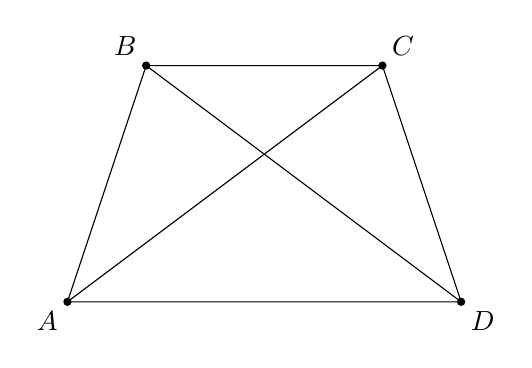
\begin{tikzpicture}[line join =round] 
		\coordinate (A) at (0,0);
		\coordinate (B) at (1,3);
		\coordinate (C) at (4,3);
		\coordinate (D) at (5,0);
		\draw (A)--(B)--(C)--(D)--cycle (D)--(B) (A)--(C);
		\fill (C) node[above right] {$C$} circle (1.5pt);
		\fill (B) node[above left] {$B$} circle (1.5pt);
		\fill (A) node[below left] {$A$} circle (1.5pt);
		\fill (D) node[below right] {$D$} circle (1.5pt);
	\end{tikzpicture}
\end{center}
\loigiai{Hình thang cân $ ABCD $ có hai cạnh bên $ AB=CD $ và hai đường chéo $ BD=AC $. \\Do đó, $ AB+BD=CD+AC>AD $.\\ Vậy 2 điểm $ B, C $ cùng thuộc một elip có hai tiêu điểm là $ A $ và $ D. $ }
\end{vd}
\begin{vd}%[0H3B3-1]
	Cho elip có phương trình chính tắc $\dfrac{x^{2}}{100}+\dfrac{y^{2}}{64}=1$. Tìm các tiêu điểm và tiêu cự của elip. Tính tổng các khoảng cách từ mỗi điểm trên elip tới hai tiêu điểm.
\loigiai{
	Ta có: $a^{2}=100, b^{2}=64$. Do đó $c=\sqrt{a^{2}-b^{2}}=6$. \\Vậy elip có hai tiêu điểm là $F_{1}(-6 ; 0) ; F_{2}(6 ; 0)$ và tiêu cự là $F_{1} F_{2}=2 c=12$. \\Ta có $a=\sqrt{100}=10$, nên tổng các khoảng cách từ mỗi điểm trên elip tới hai tiêu điểm bằng $2 a=20$.}
	\end{vd}
\subsubsection{Hypebol}
\begin{enumerate}[-]
	\item Cho hai điểm phân biệt cố định $F_{1}$ và $F_{2}$. Đặt $F_{1} F_{2}=2 c$. Cho số thực dương $ a $ nhỏ hơn $ c $. Tập hợp các điểm $M$ sao cho $\left|M F_{1}-M F_{2}\right|=2 a$ được gọi là \textbf{đường hypebol} (hay hypebol). Hai điểm $F_{1}, F_{2}$ được gọi là hai tiêu điểm và $F_{1} F_{2}=2 c$ được gọi là tiêu cự của hypebol đó.
	\item Hypebol có hai nhánh (như hình bên dưới), một nhánh gồm những điểm $M$ thoả mãn $M F_{1}-M F_{2}=2 a$ và nhánh còn lại gồm những điểm $M$ thoả mãn $M F_{1}-M F_{2}=-2 a$ (hay $\left.M F_{2}-M F_{1}=2 a\right)$.
	\begin{center}
		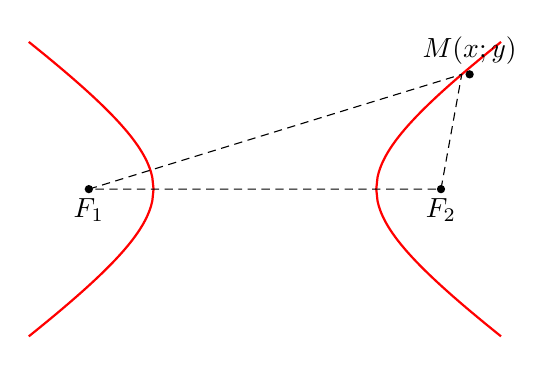
\begin{tikzpicture}
			\pgfmathsetmacro\a {sqrt(5)}
			\pgfmathsetmacro\b {sqrt(2.125)}  		
			\draw[thick,red,samples=100,domain=1.41422:3] 
			plot(\x,{sqrt(0.5*(\x)^2-1});
			\draw[thick,red,samples=100,domain=1.41422:3] 
			plot(\x,{-sqrt(0.5*(\x)^2-1});
			\draw[thick,red,samples=100,domain=-1.41422:-3] 
			plot(\x,{sqrt(0.5*(\x)^2-1});
			\draw[thick,red,samples=100,domain=-1.41422:-3] 
			plot(\x,{-sqrt(0.5*(\x)^2-1});
			\draw[densely dashed] (-\a,0)--(2.5,\b)--(\a,0)--cycle;
			\fill (2.6,\b) node[above] {$M(x;y)$} circle (1.5pt);
			\fill (-\a,0) node[below] {$F_1$} circle (1.5pt);
			\fill (\a,0) node[below] {$F_2$} circle (1.5pt);
		\end{tikzpicture}
	\end{center}
	\item Trong mặt phẳng toạ độ Oxy, hypebol có hai tiêu điểm thuộc trục hoành sao cho $O$ là trung điểm của đoạn nối hai tiêu điểm đó, thì có phương trình
	$$
	\dfrac{x^{2}}{a^{2}}-\dfrac{y^{2}}{b^{2}}=1 \text {, với } a, b>0 \text {. } \quad  \quad \quad \quad (2)
	$$
	\item Ngược lại, mỗi phương trình có dạng $ (2) $, với $a, b>0$, đều là phương trình của hypebol có hai tiêu điểm $F_{1}\left(-\sqrt{a^{2}+b^{2}} ; 0\right), F_{2}\left(\sqrt{a^{2}+b^{2}} ; 0\right)$, tiêu cự $2 c=2 \sqrt{a^{2}+b^{2}}$ và giá trị tuyệt đối của hiệu các khoảng cách từ mỗi điểm thuộc hypebol đến hai tiêu điểm bằng $2 a$.\\ Phương trình $ (2) $ được gọi là phương trình chính tắc của hypebol tương ứng.
\end{enumerate}

\begin{vd}
	Cho hypebol có phương trình chính tắc $\dfrac{x^{2}}{36}-\dfrac{y^{2}}{64}=1$. Tìm các tiêu điểm và tiêu cự của hypebol. Hiệu các khoảng cách từ một điểm nằm trên hypebol tới hai tiêu điểm có giá trị tuyệt đối bằng bao nhiêu?

\loigiai{Ta có $a^{2}=36, b^{2}=64$, nên $c=\sqrt{a^{2}+b^{2}}=10$.\\ Vậy hypebol có hai tiêu điểm là $F_{1}(-10 ; 0), F_{2}(10 ; 0)$ và có tiêu cự $2 c=20$.\\ Hiệu các khoảng cách từ một điểm nằm trên hypebol tới hai tiêu điểm có giá trị tuyệt đối bằng $2 a=2 \sqrt{36}=12$.}
\end{vd}
\begin{vd}
	Trong hệ tọa độ ${Oxy}$ cho ${A}_{1}(-{a} ; 0), {A}_{2}({a} ; 0)$. Gọi $({C})$ là đường tròn thay đổi luôn qua $A_{1}$ và $A_{2} ; MM^{\prime}$ là đường kính của $(C)$ và luôn vuông góc trục $O y$. Chứng minh rằng 2 điểm $M$ và $M^{\prime}$ luôn di động trên cùng một hypebol.
	\begin{center}
		\begin{tikzpicture}[line join =round] %câu 63
			\coordinate (O) at (0,0);
			\coordinate (I) at (0,1);
			\coordinate (M2) at (2,1);
			\coordinate (M1) at (-2,1);
			\coordinate (A1) at (-1.73205,0);
			\coordinate (A2) at (1.73205,0);
			\draw (I) circle (2) (M1)--(M2) (I)--(A1);
			\draw[-stealth] (-3,0)--(3,0)node[above]{$x$};
			\draw[-stealth] (0,-2)--(0,4)node[left]{$y$};
			\fill (M2) node[above right] {$M$} circle (1.5pt);
			\fill (M1) node[above left] {$M'$} circle (1.5pt);
			\fill (A1) node[below left] {$A_1$} circle (1.5pt);
			\fill (A2) node[below right] {$A_2$} circle (1.5pt);
			\node[below left] at (0,0) {$O$};
			\node at (-1,0.7) {$R$};
		\end{tikzpicture}
	\end{center}

\loigiai{Gọi $R$ là bán kính của đường tròn $(C)$.\\
	Ta có: $x_{M}^{2}=R^{2}=a^{2}+y_{M}^{2} \Leftrightarrow x_{M}^{2}-y_{M}^{2}=a^{2}$.\\
	Tương tự ta có: $x_{M^{\prime}}^{2}-y_{M^{\prime}}^{2}=a^{2}$.\\
	Vậy 2 điểm ${M}$ và ${M}^{\prime}$ di động trên cùng một đường hypebol $({H}): {x}^{2}-{y}^{2}={a}^{2}$.}
	\end{vd}
\subsubsection{Parabol}
\begin{enumerate}[-]
	\item Cho một điểm $F$ cố định và một đường thẳng $\Delta$ cố định không đi qua $F$. Tập hợp các điểm $M$ cách đều $F$ và $\Delta$ được gọi là \textbf{đường parabol} (hay parabol). Điểm $F$ được gọi là tiêu điểm, $\Delta$ được gọi là đường chuẩn, khoảng cách từ $F$ đến $\Delta$ được gọi là tham số tiêu của parabol đó.
	\item Xét $(P)$ là một parabol với tiêu điểm $F$, đường chuẩn $\Delta$. Gọi $H$ là hình chiếu vuông góc của $F$ trên $\Delta$. Khi đó, trong hệ trục toạ độ $O x y$ với gốc $O$ là trung điểm của $H F$, tia $O x$ trùng tia $O F$, parabol $(P)$ có phương trình
	$$
	y^{2}=2 p x \quad (\text {với} \; p>0 ). \quad  \quad \quad \quad (3)
	$$
	\item Ngược lại, mỗi phương trình dạng $(5)$, với $p>0$, là phương trình chính tắc của parabol có tiêu điểm $F\left(\dfrac{p}{2} ; 0\right)$ và đường chuẩn $\Delta: x=-\dfrac{p}{2}$.\\Phương trình $ (3) $ được gọi là phương trình chính tắc của parabol $(P)$.
	\begin{center}
		\begin{tikzpicture}
			\pgfmathsetmacro\a {0.75}
			\pgfmathsetmacro\b {sqrt(6)}
			\def\khvuong(#1,#2,#3){
				\path
				($(#2)!2mm!(#1)$) coordinate (#2#1)
				($(#2)!2mm!(#3)$) coordinate (#2#3);
				\draw (#2#1) -- ($(#2#1)+(#2#3)-(#2)$) -- (#2#3);}	
			\coordinate (M) at (2,\b);
			\coordinate (H) at (-\a,0);
			\coordinate (E) at (-\a,\b);
			\coordinate (F) at (\a,0);		
			\draw[thick,red,samples=100,domain=0:2.5] 
			plot(\x,{sqrt(3*(\x)});
			\draw[thick,red,samples=100,domain=0:2.5] 
			plot(\x,{-sqrt(3*(\x)});
			\draw (2,\b)--(\a,0)  (M)--(E); 
			\draw[orange] (-0.75,2.5)--(-0.75,-2.5);
			\draw[-stealth] (-4,0)--(4,0)node[above]{$x$};
			\draw[-stealth] (0,-3.2)--(0,3.2)node[left]{$y$};
			\fill (2,\b) node[below right] {$M(x;y)$} circle (1.5pt);
			\fill (H) node[below left] {$H$} circle (1.5pt);
			\fill (\a,0) node[below] {$F$} circle (1.5pt);
			\path 	(0,0) coordinate (O);
			\khvuong(E,H,F);		\khvuong(M,E,H);	
			\node[below left] at (0,0) {$O$};
			\node[below left] at (-\a,-2) {$\Delta$}; 
			\node[above right] at (2,-\b) {$(P)$}; 
		\end{tikzpicture}
	\end{center}
\end{enumerate}
\begin{vd}
	Cho parabol $ (P):y^2=4x $.
	\begin{enumerate}
		\item Tìm tiêu điểm $ F$, đường chuẩn $ \Delta $ của $ (P) $.
		\item Tìm các điểm $ M $ trên $ (P) $ biết $ M $ cách $ F $ một đoạn bằng 2.
	\end{enumerate}

\loigiai{
	\begin{enumerate}
		\item Ta có $2 p=4$ nên $p=2$.
		Parabol có tiêu điểm $F\left(1; 0\right)$ và đường chuẩn $\Delta: x=-1$.
		\item Điểm $M\left(x_{0} ; y_{0}\right)$ thuộc $(P)$ và có khoảng cách tới $F$ bằng $ 2 $ khi và chỉ khi $y_{0}^{2}=4x_{0}$ và $M F=2$.\\ Do $M F=d(M, \Delta)$ nên $d(M, \Delta)=2$.\\
		Mặt khác $\Delta: x+1=0$ và $x_{0}=\dfrac{y_{0}^{2}}{4} \geq 0$ nên $2=d(M, \Delta)=\left|x_{0}+1\right|=x_{0}+1$.\\
		Vậy $x_{0}=1$ và $y_{0}=2$ hoặc $y_{0}=-2$.
		Vậy có hai điểm $M$ thoả mãn bài toán với toạ độ là $\left(1 ; 2\right)$ và $\left(1 ;-2\right)$.
\end{enumerate}}
\end{vd}
% \setcounter{section}{21}
\subsection{CÁC DẠNG TOÁN THƯỜNG GẶP}
\section*{Elip}
\begin{dang}{Xác định các yếu tố của Elip}
	Nắm vững kiến thức về elip từ đó giải quyết các yêu cầu của bài toán.
\end{dang}
\vspace*{-12pt}
\subsubsection{Ví dụ minh họa}
\begin{vd}%[Nguyễn Đức Tuệ]%[0H3Y3-1]
	Trong mặt phẳng $Oxy$ cho elip $\left(E\right):{x^2}+3y^2=6$. Hãy tìm tiêu cự của Elip.
	\loigiai{
		Ta có $\left(E\right):\dfrac{x^2}{6}+\dfrac{y^2}{2}=1,$ do đó $a=\sqrt 6, \, b=\sqrt 2, \,c=2$ . Độ dài tiêu cự là $2c=4.$}
\end{vd}
\begin{vd}%[Nguyễn Đức Tuệ]%[0H3B3-1]
	Cho elip $(E)$ có độ dài trục lớn bằng $26$, tâm sai $e=\dfrac{12}{13}$. Hãy tìm độ dài trục nhỏ của $(E)$.
	\loigiai{
		Ta có $2a=26 \Rightarrow a=13$.\\
		$e=\dfrac{c}{a}=\dfrac{12}{13} \Rightarrow c=12$.\\
		$b=\sqrt{a^2-c^2}=\sqrt{169-144}=5$.\\
		Độ dài trục nhỏ là $2b=10$.}
\end{vd}
\begin{vd}%[Nguyễn Đức Tuệ]%[0H3B3-1]
	Hãy tính diện tích của tứ giác tạo nên bởi các đỉnh của elip $(E)\colon \dfrac{x^2}{4}+y^2=1$.
	\loigiai{
		Tọa độ các đỉnh của elip $(E)\colon \dfrac{x^2}{4}+y^2=1$ là $A_1(-2;0)$, $A_2(2;0)$; $B_1(0;-1)$, $B_2(0;1)$.\\
		Vì tứ giác $A_1B_1A_2B_2$ là hình thoi có hai đường chéo $A_1A_2=4$ và $B_1B_2=2$.\\
		Vậy diện tích tứ giác cần tìm là $S=\dfrac{1}{2}\cdot A_1A_2\cdot B_1B_2=4$.}
\end{vd}

\begin{vd}%[Nguyễn Đức Tuệ]%[0H3B3-1]
	Một elip $(E)$ có phương trình $\dfrac{x^2}{a^2}+\dfrac{y^2}{b^2}=1$, trong đó $a>b>0$. Biết $(E)$ đi qua điểm $A\left(2;\sqrt{2}\right)$ và $B\left(2\sqrt{2};0\right)$ hãy tìm độ dài trục bé của $ (E) $.
	\loigiai{
		\begin{itemize}
			\item $(E)$ đi qua $B\left(2\sqrt{2};0\right)$ nên ta có $\dfrac{\left(2\sqrt{2}\right)^2}{a^2}+\dfrac{0^2}{b^2}=1$ suy ra $a=2\sqrt{2}$.
			\item $(E)$ đi qua $A\left(2;\sqrt{2}\right)$ nên ta có $\dfrac{(2)^2}{8}+\dfrac{\left(\sqrt{2}\right)^2}{b^2}=1$ suy ra $b=2$.
		\end{itemize}
		Do đó độ dài trục bé $2b=4$.}
\end{vd}
\begin{vd}%[Nguyễn Đức Tuệ]%[0H3B3-1]
	Cho elip $(E)$ có hai tiêu điểm $F_1(-4;0)$, $F_2(4;0)$ và điểm $M$ thuộc $(E)$. Biết chu vi tam giác $MF_1F_2$ bằng $18$. Hãy tìm tâm sai của $(E)$.
	\loigiai{
		Ta có $F_1F_2=8$ và $c=4$.\\
		Chu vi $\triangle MF_1F_2$ là $C_{\triangle MF_1F_2}=MF_1+MF_2+F_1F_2=18 \Rightarrow MF_1+MF_2=10=2a \Rightarrow a=5$.\\
		Tâm sai của elip là $e=\dfrac{c}{a}=\dfrac{4}{5}$.}
\end{vd}
\begin{dang}{Viết phương trình chính tắc của Elip}
\end{dang}
\begin{vd}%[Nguyễn Đức Tuệ]%[0H3Y3-2] 
	Hãy viết phương trình chính tắc của $(E)$ có độ dài trục lớn bằng $8$, trục nhỏ bằng $6$.
	\loigiai{
		Ta có $\left\{
		\begin{aligned}
			&2a=8\\
			&2b=6\\
		\end{aligned}\right. $ $ \Rightarrow \left\{
		\begin{aligned}
			&a=4\\
			&b=3.
		\end{aligned}\right. $\\
		Vậy phương trình chính tắc của $(E) \colon \dfrac{x^2}{16}+\dfrac{y^2}{9}=1$.}
\end{vd}
\begin{vd}%[Nguyễn Đức Tuệ]%[0H3Y3-2] 
	Hãy viết phương trình chính tắc của $(E)$ có tâm sai $e=\dfrac{4}{5}$, độ dài trục nhỏ bằng $12$.
	\loigiai{
		Ta có $\left\{
		\begin{aligned}
			&e=\dfrac{4}{5}\\
			&2b=12\\
		\end{aligned}\right. $ $ \Leftrightarrow \left\{
		\begin{aligned}
			&5c=4a\\
			&b=6\\
		\end{aligned}\right. $ $ \Leftrightarrow \left\{
		\begin{aligned}
			&25c^2=16a^2\\
			&b=6\\
		\end{aligned}\right. $ $ \Leftrightarrow \left\{
		\begin{aligned}
			&25(a^2-b^2)=16a^2\\
			&b=6\\
		\end{aligned}\right. $ $ \Leftrightarrow \left\{
		\begin{aligned}
			&a=10\\
			&b=6.
		\end{aligned}\right. $\\
		Vậy phương trình của $(E) \colon \dfrac{x^2}{100}+\dfrac{y^2}{36}=1$.}
\end{vd}
\begin{vd}%[Nguyễn Đức Tuệ]%[0H3Y3-2]
	Trong mặt phẳng tọa độ $Oxy$, hãy viết phương trình chính tắc của đường elip có độ dài trục lớn và trục nhỏ lần lượt bằng $10$ và $8$.
	\loigiai
	{
		Ta có
		\[\heva{&2a=10 \\&2b=8} \Leftrightarrow \heva{&a=5 \\&b=4.}\]
		Vậy phương trình chính tắc của elip đã cho là $\dfrac{x^2}{25}+\dfrac{y^2}{16}=1$.
	}
\end{vd}

\begin{vd}%[Nguyễn Đức Tuệ]%[0H3Y3-2]
	Trong mặt phẳng với hệ tọa độ $Oxy$, hãy viết phương trình chính tắc của e-líp có trục lớn gấp đôi trục bé và có tiêu cự bằng $4\sqrt{3}$.
	\loigiai{
		E-líp cần tìm có dạng $\dfrac{x^2}{a^2}+\dfrac{y^2}{b^2}=1$ ($a>b>0$). Ta có
		$$\heva{& 2c=4\sqrt{3}\\ & a=2b\\ & a^2=b^2+c^2}\Leftrightarrow \heva{& c=2\sqrt{3}\\ & b^2=4\\ & a^2=16.}$$
		Vậy e-líp cần tìm là $\dfrac{x^2}{16}+\dfrac{y^2}{4}=1$.}
\end{vd}
\begin{vd}%[0H3B3-2]
	Elip có hai đỉnh $(-3;0)$; $(3;0)$ và hai tiêu điểm $(-1;0)$ và $(1;0)$, hãy viết phương trình chính tắc của Elip đã cho.
	\loigiai{
		Theo đề bài ta có $\left\{
		\begin{aligned}
			&a=3\\
			&c=1\\
		\end{aligned}\right. \Rightarrow b^2=a^2-c^2=8$.\\
		Vậy phương trình chính tắc của elip đã cho là $\dfrac{x^2}{9}+\dfrac{y^2}{8}=1$.}
\end{vd}

\begin{vd}%[Nguyễn Đức Tuệ]%[0H3B3-2]
	Hãy viết phương trình chính tắc của elip $(E)$ có độ dài trục lớn bằng $12$, độ dài trục bé bằng tiêu cự.
	\loigiai{
		$(E)$ có độ dài trục lớn bằng $12$ nên $2a=12 \Rightarrow a=6$.\\
		Độ dài trục bé bằng tiêu cự nên: $2b=2c \Rightarrow b=c$.\\
		Mà: $b^2+c^2=a^2$ nên $b^2+b^2=6^2 \Rightarrow b^2=18$.\\
		Vậy phương trình $(E)$ là $\dfrac{x^2}{36}+\dfrac{y^2}{18}=1$.}
\end{vd}

\begin{vd}%[0H3B3-2]
	Hãy viết phương trình chính tắc của elip có trục lớn bằng $10$, tâm sai $\mathrm{e}=\dfrac{3}{5}$.
	\loigiai{
		Giả sử $(E) \colon \dfrac{x^2}{a^2}+\dfrac{y^2}{b^2}=1$.\\
		Vì $(E)$ có trục lớn bằng $10$ nên $2a=10 \Rightarrow a=5$.\\
		Tâm sai	$e=\dfrac{c}{a}=\dfrac{3}{5} \Rightarrow c=3$. Do đó $b^2=a^2-c^2=5^2-3^2=16$.\\
		Vậy phương trình của $(E) \colon \dfrac{x^2}{25}+\dfrac{y^2}{16}=1$.}
\end{vd}
\begin{vd}%[Nguyễn Đức Tuệ]%[0H3B3-2]
	Hãy viết phương trình chính tắc của elip $(E)$, biết rằng $(E)$ có độ dài trục nhỏ là $2$ và một trong hai tiểu điểm là $F(3;0)$.
	\loigiai{
		Độ dài trục nhỏ bằng $2$ suy ra $2b=2 \Leftrightarrow b=1$.\\
		Một tiêu điểm là $F(3;0)$ suy ra $c=3$ hay $a^2=b^2+c^2=1+9=10$.\\
		Vậy phương trình đường elip là 
		\[(E) \colon \dfrac{x^2}{10}+\dfrac{y^2}{1}=1.\]
	}
\end{vd}
\begin{dang}{Tìm điểm trên Elip thỏa mãn điều kiện cho trước}
\end{dang}
\begin{vd}%[0H3K3-3]
	Trong mặt phẳng với hệ toạ độ $ Oxy $, cho elip $ (E):\dfrac{x^2}{100}+\dfrac{y^2}{25}=1 $. Tìm các điểm $ M\in (E) $ sao cho $ \widehat{F_1MF_2}=120^\circ $ ($ F_1 $, $ F_2 $ là hai tiêu điểm của $ (E) $).
	\loigiai{
		Ta có $ a=10 $, $ b=5 $, dễ dàng tính được $ c=5\sqrt{3} $.\\
		Gọi $ M\left(x ; y \right)\in (E)  \Rightarrow MF_1=10-\dfrac{\sqrt{3}}{2}x, MF_2=10+\dfrac{\sqrt{3}}{2}x$.\\
		$ F_1F_2^2=MF_1^2+MF_2^2-2MF_1\cdot MF_2\cdot \cos \widehat{F_1MF_2} $\\
		$ \Leftrightarrow (10\sqrt{3})^2=\left(10-\dfrac{\sqrt{3}}{2}x\right)^2+\left(10+\dfrac{\sqrt{3}}{2}x\right)^2-2\left(10-\dfrac{\sqrt{3}}{2}x\right)\left(10+\dfrac{\sqrt{3}}{2}x\right)\left(-\dfrac{1}{2}\right) $\\
		$ \Leftrightarrow x =0 $, $ y=\pm 5 $.\\
		Vậy có hai điểm thỏa mãn đề bài là $ M_1(0;5) $, $ M_2(0;-5) $.
	}
\end{vd}
\begin{vd}%[0H3K3-3]
	Cho elip $ (E):\dfrac{x^2}{25}+\dfrac{y^2}{16}=1 $, $ F_1(-3;0) $, $ F_2(3;0) $ là các tiêu điểm của $ (E) $. Xác định tọa độ
	điểm $ M \in (E) $, biết rằng $ 2MF_1=MF_2 $.
	\loigiai{
		Gọi $M\left(x_0; y_0\right)\in(E)\Rightarrow\dfrac{x_0^2}{25}+\dfrac{y_0^2}{16}=1$.\\
		Elip $(E)$ có tâm sai $e=\dfrac{c}{a}=\dfrac{3}{5}$, ta có $M F_1=a+e x_0; M F_2=a-e x_0$.\\
		$M F_2=2M F_1\Leftrightarrow a-e x_0=2\left(a+e x_0\right)$\\
		$\Leftrightarrow x_0=\dfrac{-a}{3e}=\dfrac{-5}{3\cdot\dfrac{3}{5}}=\dfrac{-25}{9}\Rightarrow y_0=\pm\dfrac{4\sqrt{56}}{9}$.\\
		Vậy $ M\left( -\dfrac{25}{9};\dfrac{4\sqrt{56}}{9}\right)  $	hoặc $ M\left( -\dfrac{25}{9};-\dfrac{4\sqrt{56}}{9}\right)  $.
	}
\end{vd}
\begin{vd}%[0H3K3-3]
	Trong mặt phẳng với hệ toạ độ $ Oxy $, cho điểm $ C(2;0) $ và elip $ (E):\dfrac{x^2}{4}+\dfrac{y^2}{1}=1 $. Tìm toạ độ
	các điểm $ A $, $ B $ thuộc $ (E) $, biết rằng hai điểm $ A $, $ B $ đối xứng với nhau qua trục hoành và tam giác $ ABC $ là tam giác đều.
	\loigiai{
		Giả sử $ A(x_0;y_0) $, $ B(x_0;y_0) \in (E)\Rightarrow \dfrac{x_0^2}{4}+\dfrac{y_0^2}{1}=1$.\quad $ (1) $\\
		Do $ C $ là một đỉnh của $ (E) $ nằm trên trục hoành, nên tam giác $ ABC $ cân tại $ C $.\\
		Tam giác ABC đều khi và chỉ khi $ \mathrm{d}(C,(AB)) =\dfrac{\sqrt{3}}{2}AB\Leftrightarrow 2-x_0=\dfrac{\sqrt{3}}{2}|y_0|$. \quad $ (2) $\\
		Từ $ (1) $ và $ (2) $ suy ra $ \heva{& x_0=\dfrac{2}{7} \\ & y_0=\pm \dfrac{4\sqrt{3}}{7}.} $\\
		Vậy $ A\left( \dfrac{2}{7};\dfrac{4\sqrt{3}}{7}\right)  $, $ B\left( \dfrac{2}{7};-\dfrac{4\sqrt{3}}{7}\right)  $ hoặc $ A\left( \dfrac{2}{7};-\dfrac{4\sqrt{3}}{7}\right)  $,  $ B\left( \dfrac{2}{7};\dfrac{4\sqrt{3}}{7}\right)  $.
	}
\end{vd}
\begin{vd}%[0H3K3-3]
	Cho elip $ (E):\dfrac{x^2}{4}+y^2=1 $ và $ A(4;-3) $, $ B(-4;3) $. Hãy tìm $ M $ thuộc $ (E) $ sao cho diện tích tam giác $ MAB $ đạt lớn nhất.
	\loigiai{
		Phương trình đường thẳng $ AB:3x+4y=0 $.\\
		Ta có $ M\in (E)\Rightarrow \heva{& x=2\cos t \\ & y=\sin t.} $\\
		Do $ AB $ cố định nên diện tích tam giác $ MAB $ đạt giá trị lớn nhất khi $ \mathrm{d}(M,(AB)) $ đạt giá trị lớn nhất, điều này tương đương $ \dfrac{|6\cos t+4\sin t|}{5} $ đạt giá trị lớn nhất $ \Leftrightarrow |5\cos t +4\sin t| $ đạt giá trị lớn nhất.\\
		Mà theo bất đẳng thức Bunhiacopxki $  |5\cos t +4\sin t| \le \sqrt{5^2+4^2}\cdot \sqrt{\cos^2t + \sin^2 t} =2\sqrt{13}$.\\
		Dấu bằng xảy ra khi $ \heva{& \dfrac{\cos t}{5}=\dfrac{\sin t}{4} \\ & |5\cos t + 4\sin t|=2\sqrt{13}} \Leftrightarrow \hoac{& \heva{& \cos t =\dfrac{3}{\sqrt{13}} \\ & \sin t = \dfrac{2}{\sqrt{13}}} \\ & \heva{& \cos t =-\dfrac{3}{\sqrt{13}}  \\ & \sin t = -\dfrac{2}{\sqrt{13}}}}\Rightarrow \hoac{& M_1\left(\dfrac{6}{\sqrt{13}}; \dfrac{2}{\sqrt{13}}\right)  \\ & M_2\left(-\dfrac{6}{\sqrt{13}}; -\dfrac{2}{\sqrt{13}}\right).}$\\
		Vậy có hai điểm $ M $ thỏa yêu cầu bài toán là $ M_1\left(\dfrac{6}{\sqrt{13}}; \dfrac{2}{\sqrt{13}}\right)  $, $ M_2\left(-\dfrac{6}{\sqrt{13}}; -\dfrac{2}{\sqrt{13}}\right) $.
	}
\end{vd}
\begin{dang}{Bài toán thực tế về Elip}
\end{dang}
\begin{vd}%[0H3K3-4]
	\immini
	{
		Ông Hoàng có một mảnh vườn hình Elip có chiều dài trục lớn và trục nhỏ lần lượt là $60$ m và $30$ m. Ông chia mảnh vườn ra làm hai nửa bằng một đường tròn tiếp xúc trong với Elip để làm mục đích sử dụng khác nhau (xem hình vẽ). Nửa bên trong đường tròn ông trồng cây lâu năm, nửa bên ngoài đường tròn ông trồng hoa màu.  Hãy tính tỉ số diện tích $T$ giữa phần trồng cây lâu năm so với diện tích trồng hoa màu. Biết diện tích hình Elip được tính theo công thức $S=\pi ab$ với $a$, $b$ lần lượt là nửa độ dài trục lớn và nửa độ dài trục bé. Biết độ rộng của đường Elip là không đáng kể.
	}
	{
		\begin{tikzpicture}[line join=round, line cap=round,thick,scale=0.8]
			\tikzset{label style/.style={font=\footnotesize}}
			\tkzDefPoints{0/0/O}
			\draw (O) circle(1.5cm);
			\draw (O) ellipse (3cm and 1.5cm);
		\end{tikzpicture}
	}
	\loigiai{
		\immini
		{
			Xét hệ trục tọa độ $Oxy$ như \textbf{hình vẽ}.\\
			Khi đó đường tròn có bán kính là $R=15$ và elip có nửa độ dài trục lớn là $a=30$, nửa độ dài trục bé là $b=15$.\\
			Diện tích đường tròn là $S_{(C)}=\pi R^2=\pi \cdot 15^2=225\pi$.\\
			Diện tích Elip là $S_{(E)}=\pi ab=\pi 30\cdot 15=450\pi$.\\
			Diện tích nửa bên ngoài đường tròn trồng hoa màu là\\ $S=S_{(E)}-S_{(C)}=450\pi -225\pi =225\pi$.\\
			Vậy tỉ số diện tích $T=\dfrac{225\pi}{225\pi}=1$.
		}
		{
			\begin{tikzpicture}[scale=0.7,>=stealth, font=\footnotesize, line join=round, line cap=round]
				\tikzset{label style/.style={font=\footnotesize}}
				\draw[->] (-4,0)--(4,0) node [below]{$x$};
				\draw[->] (0,-2)--(0,2.5) node [left]{$y$};
				\draw[fill=black] (0,0) circle(1pt) node at (0,0) [below left]{$O$};
				\draw[fill=black] (3,0) circle(1pt) node at (3,0) [below right]{\footnotesize$ 30$};
				\draw[fill=black] (-3,0) circle(1pt) node at (-3,0) [below left]{\footnotesize$-30$};
				\draw[fill=black] (0,1.5) circle(1pt) node at (0,1.5) [above right]{\footnotesize$15$};
				\draw[fill=black] (0,-1.5) circle(1pt) node at (0,-1.5) [below right]{\footnotesize$-15$};
				\clip (-4,-2) rectangle (4,2.5);
				\draw (O) circle(1.5cm);
				\draw (O) ellipse (3cm and 1.5cm);
			\end{tikzpicture}
		}
	}
\end{vd}
\section*{Hypebol}
\begin{dang}{Xác định các yếu tố của Hypebol}
\end{dang}
\begin{vd}
	Xác định độ dài hai trục, tiêu cự, tâm sai, tiêu điểm, của hypebol $(H):9x^2-16y^2-144=0$.
	\loigiai{
		$ (H):9x^2-16y^2-144=0 \Leftrightarrow \dfrac{x^2}{16}-\dfrac{y^2}{9}=1$.\\
		$ (H) $ có trục thực $ Ox $, $ a=4 $, $ b=3 $, $ c=\sqrt{4^2+3^2}=5 $.\\
		Từ đó trục thực $ 2a=8 $, trục ảo $ 2b=6 $.\\
		Tiêu cự $ 2c=10 $, tâm sai $ e=\dfrac{c}{a}=\dfrac{5}{4} $.\\
		Hai tiêu điểm $ F_1\left(-5;0 \right)  $, $ F_2\left( 5;0\right)  $.
	}
\end{vd}
\begin{vd}
	Xác định độ dài hai trục, tiêu cự, tâm sai, tiêu điểm, của hypebol $ x^2-4y^2-4=0$.
	\loigiai{
		$ (H):\dfrac{x^2}{4}-\dfrac{y^2}{1}=1 \Rightarrow \heva{& a^2=4 \\ & b^2=1}\Rightarrow c^2=a^2+b^2=5 \; (a>b)$.\\
		Trục thực $ A_1A2=2a=4 $.\\
		Trục ảo $ B_1B_2=2b=2 $.\\
		Tiêu điểm $ F_1\left( -\sqrt{5} ; 0\right) $, $ F_2\left( \sqrt{5};0\right)  $.\\
		Tâm sai $ e=\dfrac{c}{a}=\dfrac{\sqrt{5}}{2}>1 $.	
	}
\end{vd}
\begin{dang}{Viết phương trình chính tắc của Hypebol}
\end{dang}
\begin{vd}
	Trong mặt phẳng tọa độ $ Oxy $, cho hypebol $ (H) $ đi qua điểm $ M\left( 5;\dfrac{9}{4}\right)  $ và nhận điểm $ F(5;0) $ làm tiêu điểm. Hãy viết phương trình chính tắc của $ (H) $.
	\loigiai{
		Phương trình chính tắc của $ (H):\dfrac{x^2}{a^2}-\dfrac{y^2}{b^2}=1\;\; (a, b>0) $.\\
		$ F(5;0) $ làm tiêu điểm suy ra $ c=5 \Rightarrow a^2+b^2=25. \quad (1)$\\
		$ M\left( 5;\dfrac{9}{4}\right)  \in (H)\Rightarrow \dfrac{25}{a^2}-\dfrac{81}{16b^2}=1. \quad (2)$
		Từ $ (1) $ và $ (2) $ suy ra $ \heva{& a^2=16 \\ & b^2=9} $ hoặc $ \heva{& a^2=\dfrac{625}{16} \\ & b^2=-\dfrac{225}{16} \; \text{(loại).}}$\\
		Vậy phương trình chính tắc của $(H) $ là $ \dfrac{x^2}{16}-\dfrac{y^2}{9}=1$.
	}
\end{vd}
\begin{vd}
	Hypebol $ (H) $ có nửa trục thực là $ 4 $, tiêu cự bằng $ 10 $. Hãy viết phương trình chính tắc của $ (H) $.
	\loigiai{
		Hypebol $ (H) $ có nửa trục thực là $ 4 \Rightarrow a=4$.\\
		Tiêu cự $ F_1F_2=2c=10\Rightarrow c=5 $.\\
		Ta có $ b^2=c^2-a^2=9 $.\\
		Suy ra phương trình chính tắc của $ (H) $ là $ \dfrac{x^2}{16}-\dfrac{y^2}{9}=1$. 
	}
\end{vd}
\begin{vd}
	Cho hypebol $ (H) $ đi qua điểm $ (6;0) $ và có tâm sai bằng $ \dfrac{7}{6} $. Hãy viết phương trình chính tắc của hypebol $ (H) $.
	\loigiai{
		$ (H) $ đi qua $ (6;0) $ suy ra $ a=6 $.\\
		Tâm sai $ e=\dfrac{c}{a}=\dfrac{7}{6}\Rightarrow c = \dfrac{7}{6}\cdot 6=7 $.\\
		Ta có $ b^2=c^2-a^2=49-36=13$.\\
		Phương trình chính tắc của $ (H) $ là $ \dfrac{x^2}{36}-\dfrac{y^2}{13}=1 $.
	}
\end{vd}
\begin{dang}{Tìm tọa độ điểm thuộc Hypebol thỏa mãn điều kiện cho trước}
	
\end{dang}
\begin{vd}
	Cho hypebol $ (H):9x^2-y^2-9=0 $. Tìm điểm trên hypebol nhìn hai tiêu điểm dưới một góc $ \dfrac{pi}{3} $.	
	\loigiai{
		Gọi $ M(x;y) $ là  điểm thuộc $ (H) $ nhìn $ F_1 $, $ F_2 $ dưới một góc $ \dfrac{\pi}{3} $.\\
		Theo định lý cosin trong tam giác $ MF_1F_2 $ ta có \\
		$ F_1F_2^2=MF_1^2+MF_2^2-2MF_1\cdot MF_2 \cdot \cos \dfrac{\pi}{3} $\\
		$ \Rightarrow F_1F_2^2 = (MF_1-MF_2)^2+MF_1\cdot MF_2 $\\
		$ \Rightarrow 4c^2=4a^2+|ex+a|\cdot |ex-a| $\\
		$ \Rightarrow  4c^2=4a^2 +\dfrac{c^2}{a^2}x^2-a^2$\\
		$ \Rightarrow 40=4+10x^2-1\Rightarrow x^2=\dfrac{37}{10}\Rightarrow x_M=\pm \dfrac{\sqrt{370}}{10} $.\\
		$ y_M^2 =9x_M^2-9=\dfrac{243}{10}\Rightarrow y_M=\pm \dfrac{9\sqrt{30}}{10}$.\\
		Vậy có $ 4 $ điểm thỏa mãn bài toán là $ \left( \dfrac{\sqrt{370}}{10};\dfrac{9\sqrt{30}}{10}\right)  $, $ \left( \dfrac{\sqrt{370}}{10};-\dfrac{9\sqrt{30}}{10}\right)  $, $ \left(- \dfrac{\sqrt{370}}{10};\dfrac{9\sqrt{30}}{10}\right)  $, $ \left(- \dfrac{\sqrt{370}}{10};-\dfrac{9\sqrt{30}}{10}\right)  $.    	
	}
\end{vd}
\begin{vd}
	Cho Hypebol $\left( H \right):\dfrac{x^2}{4}-y^2=1$. Tìm điểm $M$ trên $\left( H \right)$ sao cho $M$ thuộc nhánh phải và $MF_1$ nhỏ nhất (ngắn nhất).
	\loigiai{
		Ta có $\heva{&a^2=4 \\&b^2=1 \\&c^2=a^2+b^2}\Rightarrow \heva{&a=2 \\&b=1 \\&c=\sqrt{5}.}$\\
		Gọi $M\left( x_0;y_0 \right)\in \left( H \right)$.\\
		Ta có $\dfrac{x^2}{4}-y^2=1\Leftrightarrow x^2=4\left( y^2+1 \right)$. $M$ thuộc nhánh phải của $\left( H \right)$ nên $x_0\ge 2$.\\
		$MF_1=2+\dfrac{2}{\sqrt{5}}x_0\ge 2+\dfrac{4}{\sqrt{5}}$.\\
		$MF_1$ nhỏ nhất bằng $2+\dfrac{4}{\sqrt{5}}$ khi $M\equiv A\left( 2;0 \right)$.}
\end{vd}

\begin{vd}
	Cho Hyperbol $\left( H \right):\dfrac{x^2}{4}-y^2=1$. Tìm điểm $M$ trên $\left( H \right)$ sao cho khoảng cách từ $M$ đến đường thẳng $\Delta:y=x+1$ đạt giá trị nhỏ nhất.
	\loigiai{
		Gọi $M\left( x_0;y_0 \right)\in \left( H \right)$. Phương trình tiếp tuyến của $\left( H \right)$ tại $M$ là $d:\dfrac{x\cdot x_0}{4}-y\cdot y_0=1$.\\
		$\Delta \parallel d$ khi $\dfrac{\dfrac{x_0}{4}}{1}=\dfrac{-y_0}{-1}\Rightarrow y_0=\dfrac{x_0}{4}$ thay vào $\left( H \right)$ ta có:
		$\dfrac{x_0^2}{4}-\left( \dfrac{x_0}{4} \right)^2=1\Leftrightarrow \hoac{&x_0=\dfrac{4}{\sqrt{3}},  y_0=\dfrac{1}{\sqrt{3}} \\&x_0=-\dfrac{4}{\sqrt{3}}, y_0=-\dfrac{1}{\sqrt{3}}.}$\\
		Với $M\left( \dfrac{4}{\sqrt{3}};\dfrac{1}{\sqrt{3}} \right)$ ta có $d\left( M,\vartriangle \right)=\dfrac{1+\sqrt{3}}{\sqrt{2}}$.\\
		Với $M\left( -\dfrac{4}{\sqrt{3}};-\dfrac{1}{\sqrt{3}} \right)$ ta có $d\left( M,\vartriangle \right)=\dfrac{\sqrt{3}-1}{\sqrt{2}}$.\\
		Vậy $ M\left( -\dfrac{4}{\sqrt{3}};-\dfrac{1}{\sqrt{3}} \right) $ thỏa mãn đề bài.
	}
\end{vd}
\section*{Parabol}
\begin{dang}{Xác định các yếu tố của Parabol}
\end{dang}
\begin{vd}
	Hãy xác định tiêu điểm, đường chuẩn, bán kính qua tiêu của parabol $ y^2=4x $.
	\loigiai{
		Từ phương trình parabol $ y^2=4x  \Rightarrow p = 2$.\\
		Tiêu điểm của parabol là $ F(1;0) $.\\
		Đường chuẩn $ \Delta: x =-1 $.\\
		Với $ M(x;y)\in (P) $ bán kính qua tiêu $ MF=x+1 $.
	}
\end{vd}
\begin{vd}
	Hãy xác định tiêu điểm, đường chuẩn, bán kính qua tiêu của parabol $ y^2=6x $.
	\loigiai{
		Từ phương trình parabol $ y^2=6x  \Rightarrow p = 3$.\\
		Tiêu điểm của parabol là $ F\left( \dfrac{3}{2};0\right) $.\\
		Đường chuẩn $ \Delta: x =-\dfrac{3}{2}$.\\
		Với $ M(x;y)\in (P) $ bán kính qua tiêu $ MF=x+ \dfrac{3}{2}$.
	}
\end{vd}
\begin{dang}{Viết phương trình chính tắc của parabol}
\end{dang}
\begin{vd}
	Hãy viết phương trình chính tắc của Parabol biết đường chuẩn có phương trình $ x + 1 = 0 $.
	\loigiai{
		Phương trình đường chuẩn $ x=-1 \Rightarrow -\dfrac{p}{2}=-1\Rightarrow p=2$.\\
		Phương trình chính tắc của parabol là $ y^2=4x $.
	}
\end{vd}
\begin{vd}
	Viết phương trình chính tắc của Parabol $ (P) $ có tiêu điểm $ F(3 ; 0) $ và đỉnh là gốc tọa độ $ O $.
	\loigiai{
		Phương trình chính tắc của $ (P) $ là $ y^2=2px $.\\
		Tiêu điểm $ F(3;0)\Rightarrow \dfrac{p}{2}=3\Rightarrow p=6 $.\\
		Phương trình chính tắc của $ (P) $ là $ y^2=12x $.
	}
\end{vd}
\begin{dang}{Xác định tọa độ điểm thuộc parabol thỏa mãn điều kiện cho trước}
\end{dang}
\begin{vd}
	Cho parabol $ (P):y^2=4x $. Tìm tọa độ điểm $ M $ thuộc $ (P) $ sao cho $ MF=3 $.
	\loigiai{
		Phương trình $ (P):y^2=4x \Rightarrow p=2$.\\
		Ta có $ MF=x_M+1=3\Rightarrow x_M =2\Rightarrow y=\pm 2\sqrt{2} $.\\
		Vậy có hai điểm $ M $ thỏa đề bài là $ M_1\left( 2;2\sqrt{2}\right)  $, $ M_2\left( 2;-2\sqrt{2}\right)  $.
	}
\end{vd}
\begin{vd}
	Trong mặt phẳng tọa độ $ Oxy $ cho parabol $ (P):y^2=x $ và điểm $ I(0;2) $. Xác định tọa độ hai
	điểm $ M $, $ N \in (P)$ sao cho $ \overrightarrow{IM}=4\overrightarrow{IN} $.\\
	\loigiai{
		Dựa vào hình dáng đồ thị parabol $ (P) $ suy ra $ M(x_M ; -\sqrt{x_M}) $, $ N(x_N ; \sqrt{x_N}) $ ($ x_M, x_N >0 $).\\
		$ \overrightarrow{IM}=4\overrightarrow{IN} \Leftrightarrow \heva{& x_M-0=4(x_N-0) \\ & -\sqrt{x_M}-2=4\left( \sqrt{x_N}-2\right) }\Leftrightarrow \heva{& x_M-4x_N=0 \\ & \sqrt{x_M}+4\sqrt{x_N}=6.}$\\
		Giải hệ phương trình ta được:\\
		$ x_N=1 $ và $ x_M=4 $ suy ra $ M(4;-2) $, $ N(1;1) $.\\
		$ x_N=9 $ và $ x_M=36 $ suy ra $ M(36;-6) $, $ N(9;3) $.
	}
\end{vd}
\begin{vd}
	Cho parabol $ (P):y^2=4x $ và đường thẳng $ (d):x+y+m=0 $ cắt $ (P) $ tại hai điểm phân biệt $ A $ và $ B $. Viết phương trình đường thẳng $ (d) $, biết rằng $ OA\perp OB $.
	\loigiai{
		Phương trình hoành độ giao điểm của $ (P) $ và $ (d) $ là $ x^2+2(m-2)x+m^2=0 $.\quad (*)\\
		$ (d) $ và $ (P) $ cắt nhau tại hai điểm $ A $ và $ B $ nên $ (*) $ có hai nghiệm phân biệt\\
		$ \Leftrightarrow \Delta'=(m-2)^2-m^2>0 \Leftrightarrow -4m+4>0\Leftrightarrow m<1.\quad (1)$\\
		Phương trình $ (*) $ có hai nghiệm phân biệt $ x_1 $, $ x_2 $ thì $ A\left( x_1;-x_1-m\right) $, $ B\left( x_2;-x_2-m\right)  $.\\
		$ OA\perp OB \Rightarrow \overrightarrow{OA}\cdot \overrightarrow{OB}=0\Leftrightarrow x_1\cdot x_2 +(x_1+m)(x_2+m)=0$ \\
		$ \Leftrightarrow 2x_1x_2 +m(x_1+x_2)+m^2=0 \Leftrightarrow 2m^2+2m(m-2)+m^2=0\Leftrightarrow 5m^2-4m=0\Leftrightarrow \hoac{& m=0 \\ & m=\dfrac{4}{5}.}$\\
		Kết hợp với điều kiện (1) ta nhận $ \hoac{& m=0 \\ & m=\dfrac{4}{5}.}$
	} 
\end{vd}
\subsection{BÀI TẬP TỰ LUẬN}
\begin{bt}%[7.19 sách kết nối]%[0H3B3-1]
	Cho elip có phương trình $\dfrac{x^{2}}{36}+\dfrac{y^{2}}{9}=1$. Tìm tiêu điểm và tiêu cự của elip.
	\loigiai{
		Elip có phương trình $\dfrac{x^{2}}{36}+\dfrac{y^{2}}{9}=1\Rightarrow\heva{&a=6\\&b=3.}$	\\
		Suy ra $c=\sqrt{a^2-b^2}=3\sqrt{3}$. Khi đó elip có 2 tiêu điểm là $F_1\left(3\sqrt{3};0\right)$ và $F_2\left(-3\sqrt{3};0\right)$. Tiêu cự là $F_1F_2=2c=6\sqrt{3}$.
	}
\end{bt}
\begin{bt}%[7.20 sách kết nối]
	Cho hypebol có phương trình $\dfrac{x^2}{7}-\dfrac{y^2}{9}=1$. Tìm tiêu điểm và tiêu cự của hypebol.
	\loigiai{
		Hypebol có phương trình $\dfrac{x^2}{7}-\dfrac{y^2}{9}=1\Rightarrow\heva{&a=\sqrt{7}\\&b=3.}$	\\
		Suy ra $c=\sqrt{a^2+b^2}=4$. Khi đó hypebol có 2 tiêu điểm là $F_1\left(4;0\right)$ và $F_2\left(-4;0\right)$. Tiêu cự là $F_1F_2=2c=8$.	
	}
\end{bt}
\begin{bt}%[7.21 sách kết nối]
	Cho parabol có phương trình $y^{2}=8x$. Tìm tiêu điểm và đường chuẩn của parabol.	
	\loigiai{
		Parabol có phương trình $y^{2}=8x\Rightarrow 2p=8\Rightarrow p=4.$\\
		Khi đó parabol có tiêu điểm là $F\left(2;0\right)$. Đường chuẩn của parabol là $x=-2$.	
	}
\end{bt}
\begin{bt}%[7.22 sách kết nối]%[0H3B3-2]
	Lập phương trình chính tắc của elip đi qua điểm $A(5;0)$ và có một tiêu điểm là $F_{2}(3 ; 0)$.
	\loigiai{
		Vì elip có một tiêu điểm là $F_{2}(3 ; 0)$ nên $c=3\Leftrightarrow a^2-b^2=9$.\\
		Gọi phương trình chính tắc của elip là $\dfrac{x^2}{a^2}+\dfrac{y^2}{b^2}=1$. Vì elip đi qua điểm $A(5;0)$ nên ta có phương trình $\dfrac{25}{a^2}=1\Rightarrow a=5$.\\
		Vì $a^2-b^2=9$ nên $b^2=16\Rightarrow b=4$. Vậy phương trình chính tắc của elip là $\dfrac{x^2}{25}+\dfrac{y^2}{16}=1$.	
	}
\end{bt}
\begin{bt}%[7.23 sách kết nối]
	Lập phương trình chính tắc của parabol đi qua điểm $M(2;4)$.	
	\loigiai{
		Gọi phương trình chính tắc của parabol có dạng $y^2=2px$ với $p>0$.\\
		Vì parabol đi qua điểm $M(2;4)$ nên ta có phương trình $16=4p\Rightarrow p=4$. Vậy phương trình chính tắc của parabol có dạng $y^2=8x$
	}
\end{bt}
\begin{bt}%[7.24 sách kết nối]
	Có hai trạm phát tín hiệu vô tuyến đặt tại hai vị trí $A$, $B$ cách nhau $300 \mathrm{~km}$. Tại cùng một thời điểm, hai trạm cùng phát tín hiệu với vận tốc $292000 \mathrm{~km} / \mathrm{s}$ để một tàu thuỷ thu và đo độ lệch thời gian. Tín hiệu từ $A$ đến sớm hơn tín hiệu từ $B$ là $0,0005 \mathrm{~s}$. Từ thông tin trên, ta có thể xác định được tàu thuỷ thuộc đường hypebol nào? Viết phương trình chính tắc của hypebol đó theo đơn vị kilômét.
	\loigiai{
		Hai trạm phát tín hiệu vô tuyến đặt tại hai vị trí $A$, $B$	chính là hai tiêu điểm của hypebol. Khi đó $AB=300 \mathrm{~km}$ chính là tiêu cự của hypebol. Suy ra $2c=300\Rightarrow c=150$.\\
		Vì tàu thuỷ thuộc đường hypebol và tín hiệu từ $A$ đến sớm hơn tín hiệu từ $B$ là $0,0005 \mathrm{~s}$ nên $\left| MF_1
		-MF_2\right| =0,0005\cdot 292000=146=2a\Rightarrow a=73.$\\
		Khi đó $b^2=c^2-a^2=150^2-73^2=17171$.\\
		Phương trình chính ủa hypebol đó theo đơn vị kilômét là $\dfrac{x^2}{5329}-\dfrac{y^2}{17171}=1$.
		
	}
\end{bt}
\begin{bt}%[7.25 sách kết nối]
	\immini{Khúc cua của một con đường có dạng hình parabol, điểm đầu vào khúc cua là $A$, điểm cuối là $B$, khoảng cách $AB=400 \mathrm{~m}$. Đỉnh parabol $\left(P\right)$ của khúc cua cách đường thẳng $AB$ một khoảng $20 \mathrm{~m}$ và cách đều $A$, $B$.
		\begin{enumerate}[a.]
			\item Lập phương trình chính tắc của $\left(P\right)$, với 1 đơn vị đo trong mặt phẳng toạ độ tương ứng $1 \mathrm{~m}$ trên thực tế.
			\item Lập phương trình chinh tắc của $\left(P\right)$, với 1 đơn vị đo trong mặt phẳng toạ độ tương ứng $1 \mathrm{~km}$ trên thực tế.
	\end{enumerate}}{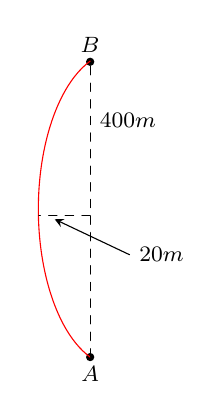
\begin{tikzpicture}[>=stealth,line join=round,line cap=round,font=\footnotesize,scale=1]
			\coordinate[label=below :$A$](A) at (2,0); 
			\coordinate[label=above:$B$](B) at (2,3.75);
			\coordinate[label=right:$400 m$](400m) at (2,3);	
			\coordinate[label=right:$20 m$](20m) at (2.5,1.3);
			\fill[black] (A) circle (1.5pt) (B) circle (1.5pt);
			
			\draw[red] (2,0) arc (250:110:1cm and 2cm); 
			\draw[dashed] (2,0)--(2,3.7) (2,1.8)--(1.35,1.8);
			\draw[->] (2.5,1.3)--(1.55,1.75);
			
	\end{tikzpicture}}
	
	\loigiai{
		\immini{ a. Chọn hệ trục toa độ $Oxy$ như hình vẽ, với 1 đơn vị đo trong mặt phẳng toạ độ tương ứng $1 \mathrm{~m}$ trên thực tế.\\
			Gọi phương trình chính tắc của parabol có dạng $y^2=2px$ với $p>0$.\\
			Vì parabol đi qua điểm $B(20;200)$ nên ta có phương trình $200^2=40p\Rightarrow p=1000$.\\
			Vậy phương trình chính tắc của parabol có dạng $y^2=2000x$.}{
			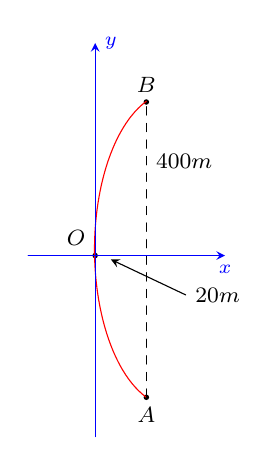
\begin{tikzpicture}[>=stealth,line join=round,line cap=round,font=\footnotesize,scale=1]
				\coordinate[label=below :$A$](A) at (2,0); 
				\coordinate[label=above:$B$](B) at (2,3.75);
				\coordinate[label=above left:$O$](O) at (1.35,1.8);
				\coordinate[label=right:$400 m$](400m) at (2,3);	
				\coordinate[label=right:$20 m$](20m) at (2.5,1.3);
				\fill[black] (A) circle (1pt) (B) circle (1pt) (O) circle (1pt);
				\draw[red] (2,0) arc (250:110:1cm and 2cm); 
				\draw[dashed] (2,0)--(2,3.7) (2,1.8)--(1.35,1.8);
				\draw[->] (2.5,1.3)--(1.55,1.75)  ;
				\draw[blue,->] (0.5,1.8)--(3,1.8) node[below] {\scriptsize $x$};
				\draw[blue,->] (1.35,-0.5)--(1.35,4.5) node[right] {\scriptsize $y$};
		\end{tikzpicture}}
		\immini{b. Chọn hệ trục toa độ $Oxy$ như hình vẽ, với 1 đơn vị đo trong mặt phẳng toạ độ tương ứng $1 \mathrm{~km}$ trên thực tế.\\
			Gọi phương trình chính tắc của parabol có dạng $y^2=2px$ với $p>0$.\\
			Vì parabol đi qua điểm $B(0,02;0,2)$ nên ta có phương trình $0,2^2=0,04p\Rightarrow p=1$.\\
			Vậy phương trình chính tắc của parabol có dạng $y^2=2x$.}{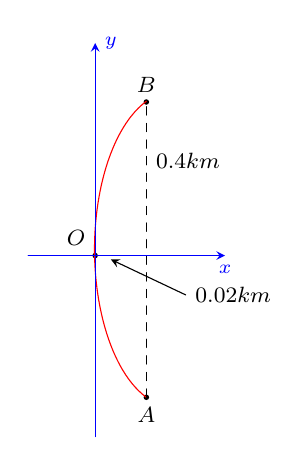
\begin{tikzpicture}[>=stealth,line join=round,line cap=round,font=\footnotesize,scale=1]
				\coordinate[label=below :$A$](A) at (2,0); 
				\coordinate[label=above:$B$](B) at (2,3.75);
				\coordinate[label=above left:$O$](O) at (1.35,1.8);
				\coordinate[label=right:$0.4 km$](400m) at (2,3);	
				\coordinate[label=right:$0.02 km$](20m) at (2.5,1.3);
				\fill[black] (A) circle (1pt) (B) circle (1pt) (O) circle (1pt);
				\draw[red] (2,0) arc (250:110:1cm and 2cm); 
				\draw[dashed] (2,0)--(2,3.7) (2,1.8)--(1.35,1.8);
				\draw[->] (2.5,1.3)--(1.55,1.75)  ;
				\draw[blue,->] (0.5,1.8)--(3,1.8) node[below] {\scriptsize $x$};
				\draw[blue,->] (1.35,-0.5)--(1.35,4.5) node[right] {\scriptsize $y$};
		\end{tikzpicture}}
	}
\end{bt}
\begin{bt}%[0H3Y3-2]
	Phương trình nào sau đây là phương trình chính tắc của elip?\\
	a) $\dfrac{x^2}{64}+\dfrac{y^2}{64}=1$; ~~~~~
	b) $\dfrac{x^2}{64}-\dfrac{y^2}{64}=1$;~~~~~
	c)$\dfrac{x^2}{64}+\dfrac{y^2}{25}=1$;~~~~~
	d) $\dfrac{x^2}{25}+\dfrac{y^2}{64}=1$.
	\loigiai 
	{	$\dfrac{x^2}{64}+\dfrac{y^2}{64}=1$ là phương trình đường tròn.\\
		$\dfrac{x^2}{64}-\dfrac{y^2}{64}=1$ là phương trình hypebol.\\
		$\dfrac{x^2}{64}+\dfrac{y^2}{25}=1$ là phương trình chính tắc của eip với $a=8, b=5$.\\
		$\dfrac{x^2}{25}+\dfrac{y^2}{64}=1$ không phải là phương trình chính tắc elip vì $a<b$.
	}
\end{bt}
\begin{bt}%[0H3B3-3]
	Cho elip $(E)$ có phương trình chính tắc là $\dfrac{x^2}{49}+\dfrac{y^2}{25}=1$. Tìm tọa độ giao điểm của elip $(E)$ với các trục tọa độ $Ox, Oy$ và tọa độ các tiêu điểm của $(E)$.
	\loigiai 
	{
		Ta có $a=7, b=5, c=\sqrt{7^2-5^2}=2\sqrt{6}$.\\
		Tọa độ giao điểm của $(E)$ với $Ox$ là $A_1(-7;0)$ và $A_2(7;0)$.\\
		Tọa độ giao điểm của $(E)$ với $Oy$ là $B_1(0;-5)$ và $B_2(0;5)$.\\
		Tiêu điểm của $(E)$ là $F_1(-2\sqrt{6};0)$ và $F_2(2\sqrt{6};0)$.
	}
\end{bt}
\begin{bt}%[0H3B3-2]
	Viết phương trình chính tắc của elip $(E)$, biết tọa độ hai giao điểm của $(E)$ với $Ox, Oy$ lần lượt là $A_1(-5;0)$ và $B_2(0;\sqrt{10})$.
	\loigiai 
	{
		Phương trình chính tắc $(E)$ có dạng $\dfrac{x^2}{a^2}+\dfrac{y^2}{b^2}=1, ~~(a>b>0)$.\\
		Ta có $(E)$ giao với $Ox, Oy$ lần lượt là $A_1(-5;0)$ và $B_2(0;\sqrt{10})$ nên $a=5$ và $b=\sqrt{10}$.\\
		Vậy phương trình chính tắc của $(E)$ là $\dfrac{x^2}{25}+\dfrac{y^2}{10}=1, ~~(a>b>0)$.
	}
\end{bt}
\begin{bt}%[0H3B3-4]
	Ta biết rằng Mặt Trăng chuyển động quanh Trái Đất theo quỹ đạo là một elip mà Trái Đất là một tiêu điểm. Elip đó có $A_1A_2= 768 800$ km và $B_1B_2=767 619$ km (Hình 62). Viết phương trình chính tắc của elip đó. 
	\begin{center}
		\begin{tikzpicture}[>=stealth,x=1cm,y=1cm,scale=.6]
			\coordinate[label=below left:$\scriptsize O$](O) at (0,0);
			\draw[->] (-7,0) -- (7,0) node[below] {$x$};
			\draw[->] (0,-3) -- (0,3) node[left] {$y$};
			\draw (O) ellipse (5cm and 2cm); % Vẽ đường elip tâm O có trục lớn 4cm và trục nhỏ 2cm
			\fill (-5,0) node [above left]{$A_1$} circle (1.5pt);
			\fill (5,0) node [above right]{$A_2$} circle (1.5pt);
			\fill (0,-2) node [below right]{$B_1$} circle (1.5pt);
			\fill (0,2) node [above right]{$B_2$} circle (1.5pt);
			\fill (-3,0) node [above]{Trái Đất} circle (4pt);
			\coordinate (A) at ($(0,0)+(60:5cm and 2cm)$);
			\fill (A) node [above right]{Mặt Trăng} circle (4pt);
			\fill (0,-5) node []{Hình 62};
		\end{tikzpicture}
	\end{center}
	\loigiai 
	{
		Ta có $A_1A_2= 768 800$ km và $B_1B_2=767 619$ km nên $a=384400$ và $b=\dfrac{767619}{2}$.\\
		Vậy phương trình chính tắc của $(E)$ là $\dfrac{x^2}{384400^2}+\dfrac{4y^2}{767619^2}=1$.
		
	}
\end{bt}
\begin{bt}
	Phương trình nào sau đây là phương trình chính tắc của hypebol?\\	
	a) $\dfrac{x^2}{9}+\dfrac{y^2}{9}=1$; ~~~~~
	b) $\dfrac{x^2}{9}-\dfrac{y^2}{9}=1$;~~~~~
	c) $\dfrac{x^2}{9}-\dfrac{y^2}{64}=1$;~~~~~
	d) $\dfrac{x^2}{64}-\dfrac{y^2}{9}=1$.
	\loigiai 
	{
		$\dfrac{x^2}{9}+\dfrac{y^2}{9}=1$ là phương trình đường tròn.\\
		$\dfrac{x^2}{9}+\dfrac{y^2}{9}=1$ là phương trình chính tắc của hypebol.\\
		$\dfrac{x^2}{9}-\dfrac{y^2}{64}=1$ là phương trình chính tắc của hypebol.\\
		$\dfrac{x^2}{64}-\dfrac{y^2}{9}=1$ là phương trình chính tắc của hypebol.
	}
\end{bt}
\begin{bt}
	Tìm tọa độ các đỉnh và tiêu điểm của hypebol trong các trường hợp sau:\\
	a) $\dfrac{x^2}{9}-\dfrac{y^2}{16}=1$;~~~~~~~~~~~~~~~~~~~~~~~~~~~~~~~~~~~~~~~~~~~~~
	b) $\dfrac{x^2}{36}-\dfrac{y^2}{25}=1$.
	\loigiai 
	{
		a) $\dfrac{x^2}{9}-\dfrac{y^2}{16}=1$.\\
		Ta có $a^2=9\rightarrow a=3,  ~~b^2=16 \rightarrow b=4$.\\
		$c=\sqrt{a^2+b^2}=5$.\\
		Tọa độ các đỉnh: $A_1(-3;0), A_2(3;0)$.\\
		Tọa độ tiêu điểm: $F_1(-5;0),~~F_2(5;0)$.
		a) $\dfrac{x^2}{36}-\dfrac{y^2}{25}=1$.\\
		Ta có $a^2=36\rightarrow a=6,  ~~b^2=25 \rightarrow b=5$.\\
		$c=\sqrt{a^2+b^2}=\sqrt{61}$.\\
		Tọa độ các đỉnh: $A_1(-6;0), A_2(6;0)$.\\
		Tọa độ tiêu điểm: $F_1(-\sqrt{61};0),~~F_2(\sqrt{61};0)$.
	}
\end{bt}
\begin{bt}
	Viết phương trình chính tắc hypebol $(H)$, biết $N(\sqrt{10};2)$ nằm trên $(H)$ và hoành độ một giao điểm của $(H)$ với $Ox$ bằng $3$.
	\loigiai 
	{
		Phương trình chính tắc của $(H)$ có dạng $\dfrac{x^2}{a^2}-\dfrac{y^2}{b^2}=1$.\\
		Một giao điểm của $(H)$ với $Ox$ bằng $3$ nên $a=3$.\\
		Khi đó $\dfrac{x^2}{9}-\dfrac{y^2}{b^2}=1$.\\
		Điểm $N(\sqrt{10};2)$ nằm trên $(H)$ nên $\dfrac{10}{9}-\dfrac{4}{b^2}=1 \Leftrightarrow \dfrac{4}{b^2}=\dfrac{1}{9}\Leftrightarrow b^2=36 \Rightarrow b=6$.\\
		Vậy $\dfrac{x^2}{9}-\dfrac{y^2}{36}=1$.
	}
\end{bt}
\begin{bt}
	Những phương trình nào sau đây là phương trình chính tắc của parabol?\\	
	a) $y^2=-2x$; ~~~~~
	b) $y^2=2x$;~~~~~
	c) $x^2=-2y$;~~~~~
	d) $y^2=\sqrt{5}x$.
	\loigiai 
	{
		a) $y^2=-2x$ không phải là phương trình chính tắc của parabol.\\
		b) $y^2=2x$ là phương trình chính tắc của parabol.\\
		c) $x^2=-2y$ không phải là phương trình chính tắc của parabol.\\
		d) $y^2=\sqrt{5}x$ là phương trình chính tắc của parabol.
	}
\end{bt}
\begin{bt}
	Tìm tọa độ tiêu điểm và viết phương trình đường chuẩn của đường parabol trong mỗi trường hợp sau:\\
	a) $y^2=\dfrac{5x}{2}$;~~~~~~~~~~~~~~~~~~~~~~~~~~~~~~~~~~~~~~~~~~~~~
	b) $y^2=2\sqrt{2}x$.
	\loigiai 
	{
		a) $y^2=\dfrac{5x}{2}$.\\
		Ta có $2p=\dfrac{5}{2}\Leftrightarrow p=\dfrac{5}{4}$.\\
		Tọa độ tiêu điểm là $F\left( \dfrac{5}{8};0\right)$.\\
		Phương trình đường chuẩn là $x+\dfrac{5}{8}=0$.\\
		b) $y^2=2\sqrt{2}x$.\\
		Ta có $2p=2\sqrt{2}\Leftrightarrow p=\sqrt{2}$.\\
		Tọa độ tiêu điểm là $F\left( \dfrac{\sqrt{2}}{2};0\right)$.\\
		Phương trình đường chuẩn là $x+\dfrac{\sqrt{2}}{2}=0$.	
	}
\end{bt}
\begin{bt}
	Viết phương trình chính tắc của parabol, biết tiêu điểm $F(6;0)$.
	\loigiai
	{
		Phương trình chính tắc của parabol có dạng $y^2=2px$.\\
		Tiêu điểm $F(6;0)$ nên $p=12$.\\
		Phương trình chính tắc của parabol có dạng $y^2=24x$.
	}
\end{bt}
\begin{bt}
	Một chiếc đèn có mặt cắt ngang là hình parabol (hình 63). Hình parabol có chiều rộng hai mép vành là $AB=40$ cm và chiều sâu $h=30$ cm ($h$ bằng khoảng cách từ $O$ đến $AB$). Bóng đèn nằm ở tiêu điểm $S$. Viết phương trình chính tắc của parabol đó.
	\begin{center}
		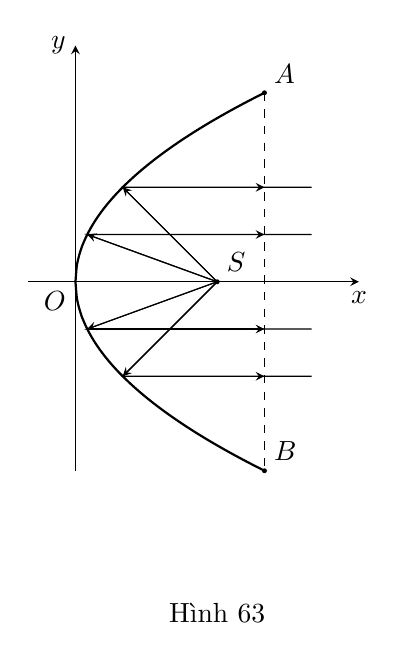
\begin{tikzpicture}[>=stealth,x=1cm,y=1cm,scale=.6]
			\coordinate[label=below left:$\scriptsize O$](O) at (0,0);
			\draw[->] (-1,0) -- (6,0) node[below] { $x$};
			\draw[->] (0,-4) -- (0,5) node[left] {$y$};
			\draw[thick,samples=150,smooth,domain=0:4] plot(\x,{2*\x^.5});
			\draw[thick,samples=150,smooth,domain=0:4] plot(\x,{-2*\x^.5});
			\fill (3,0)node[above right]{$S$} circle(1.5pt);
			\fill (4,4)node[above right]{$A$} circle(1.5pt);
			\fill (4,-4)node[above right]{$B$} circle(1.5pt);
			\draw[dashed](4,4)--(4,-4);
			\draw(5,-2)--(1,-2)--(3,0)--(1,2)--(5,2);
			\draw(5,-1)--(.25,-1)--(3,0)--(.25,1)--(5,1);
			\draw[->](.25,1)--(4,1);
			\draw[->](1,2)--(4,2);
			\draw[->](.25,-1)--(4,-1);
			\draw[->](1,-2)--(4,-2);
			\draw[->](3,0)--(.25,1);
			\draw[->](3,0)--(.25,-1);
			\draw[->](3,0)--(1,2);
			\draw[->](3,0)--(1,-2);
			\fill (3,-7)node[]{Hình 63};
		\end{tikzpicture}
	\end{center}
	\loigiai 
	{
		Phương trình chính tắc của parabol có dạng $y^2=2px$.\\
		Từ dữ kiện bài toán ta có được parabol đi qua điểm $A(30;20)$ nên $20^2=2.p.30 \Leftrightarrow p=\dfrac{20}{3}$.\\
		Vậy phương trình chính tắc của parabol là $y^2=\dfrac{40}{3}x$
	}
\end{bt}
\Closesolutionfile{ans}





